\documentclass[a4paper,12pt]{article}
\usepackage[utf8]{inputenc}
%\usepackage[latin1]{inputenc}
\usepackage{epsfig,epic,eepic,amssymb}
\graphicspath{{FIG/}{PS/}}
\usepackage[francais]{babel}
\usepackage{amssymb}
\usepackage{moreverb}
\usepackage{listings}
\lstset{language=caml, extendedchars=true}
\newtheorem{theorem}{Theorem}

\setlength{\parindent}{0pt}
\setlength{\parskip}{3mm}


\usepackage{graphicx}
\usepackage{amsfonts}
\def\commentaire#1{}
\def\C{\mathbb{C}}
\def\N{\mathbb{N}}
\def\Z{\mathbb{Z}}
\def\R{\mathbb{R}}

\begin{document}
\title{EXAMEN 2017 INFO 31, 20 décembre 2017}
\date{}
\maketitle
Répondez {\bf DANS L'ORDRE} aux questions. Répondez à chaque question soit {\bf EN UNE LIGNE} soit avec un dessin. {\bf AUCUNE PREUVE N'EST DEMANDÉE.} Ecrivez 
{\bf LISIBLEMENT} SVP.

Question 1. Calculez le PGCD $g$ et les coefficients de Bezout $u$ et $v$ de $a=84$ et $b=48$, avec le tableau habituel.
Dans la dernière ligne,  $v$ vaut $k\in\Z$.
Que valent $g$,  $u$ et $v$ ($u$ et $v$ sont des fonctions de $k$) dans la première ligne de votre tableau~? 

Question 2. Considérer l'équation en $x$~: $7^{\log_2 n}=n^x$.  Que vaut $x$~?

Question 3. La séquence commune la plus longue entre $U=CABCAB$ et $V=ACBCBA$ 
est le chemin critique d'un graphe orienté. Dessinez le graphe et son chemin critique.
Rappel~: les sommets
du graphe sont les couples $(i, j)$ tels que $U_i=V_j$. Il y a un arc  de $(i_1, j_1)$ à
$(i_2, j_2)$ ssi $i_1 < i_2$ et $j_1< j_2$. Ne tracez pas les arcs inutiles. 
Les arcs doivent aller de gauche à droite en montant.
Vous pouvez ajouter une source et un puits virtuels~; la durée de leurs arcs est nulle.
Tous les autres arcs ont comme durée 1.
Calculez les dates au plus tôt et au plus tard des sommets du graphe. Mettez en évidence le chemin critique.

Question 4. Trouvez par programmation dynamique la solution optimale de ce problème de sac à dos, avec un poids maximal de 5.
%, à l’aide de la programmation dynamique, au problème du sac à dos suivant pour un poids maximal de 15 : 
\begin{center}\begin{tabular}{|c|c|c|c|c|}\hline
article $i$ & 	0 & 	1 & 	2 & 	3\\\hline
poids $p_i$ & 	2 & 	1 & 	3 & 	2\\\hline
utilité  $u_i$ & 	12 & 	10 & 	20 & 	15\\\hline
\end{tabular}\end{center}
Vous remplirez le tableau~: $U(p,i)$ ci-dessous. Par définition, $U(p,i)$ est la plus grand utilité des sac à dos utilisant les articles dans $\{1, \ldots i\}$ et de poids inférieur ou égal à $p$. 
%% Rappel~: $U(p, 0)$ vaut $0$ si $u_0>p$ et $u_0$ sinon~; $U(p, i>0)$ vaut $U(p, i-1)$ si $p_i>p$ et $\max( U(p, i-1), u_i+ U(p-p_i, i-1))$ sinon.
\begin{center}\begin{tabular}{|c|c|c|c|c|}\hline
U(p,i) &       i=1 &     i=2 &     i=3 &     i=4\\\hline
p=1 & & & & \\\hline
p=2 & & & & \\\hline
p=3 & & & & \\\hline
p=4 & & & & \\\hline
p=5 & & & & \\\hline
\end{tabular}\end{center}
%[|[|0; 0; 0; 0|]; [|0; 10; 10; 10|]; [|12; 12; 12; 15|]; [|12; 22; 22; 25|]; [|12; 22; 30; 30|]; [|12; 22; 32; 37|]|]



\commentaire{Question 4. Dessinez le graphe réduit (sous-entendu~: des composantes fortement connexes) de ce graphe. Etiquetez-en les sommets avec les numéros des sommets du graphe initial. Tous les arcs du graphe réduit  doivent aller de gauche à droite.
\begin{center}
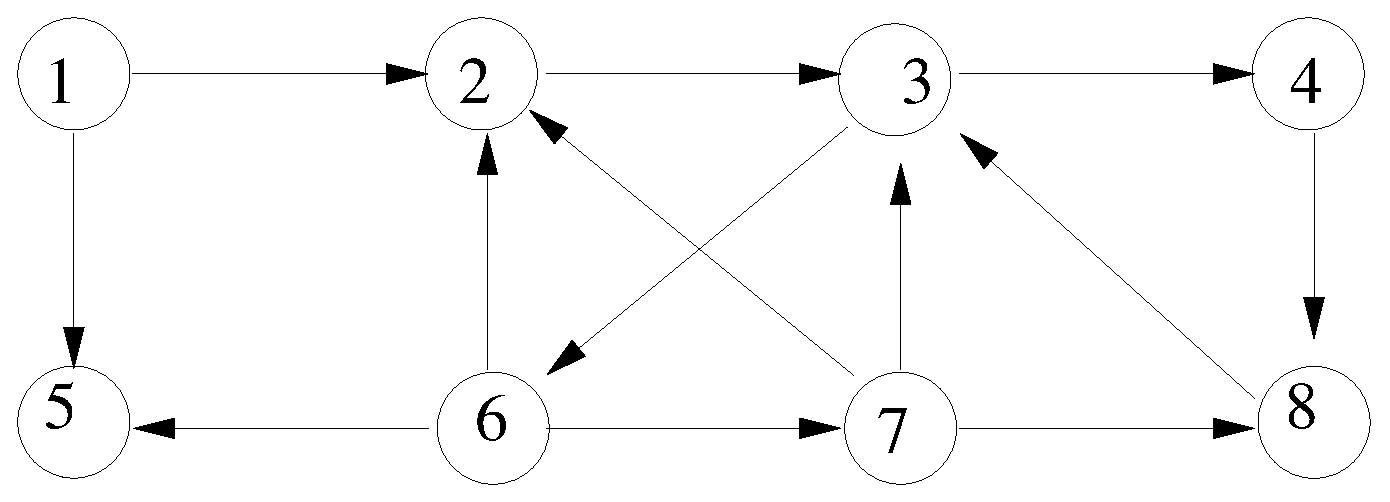
\includegraphics[width=0.55\linewidth]{graphe2017.eps}
\end{center}
}

%Question 1. Citer deux problèmes indécidables en informatique.


Question 5. Soient $(n_i\in\N, t_i=T(n_i)\in \R)$ pour $i=1, \ldots N$. Les $n_i$ sont les
tailles des données de test pour un programme, et les $t_i$ sont les temps que met le programme pour calculer avec $n_i$ données.  
%Les points $(n_i, t_i)$ 
%sont affichés dans un diagramme log-log~: autrement dit, 
Les points de coordonnées $(x_i=\log_2 n_i, y_i=\log_2 t_i)$ sont affichés.
Si $T(n)=n^d$, quelle est l'équation de la courbe
sur laquelle se trouvent les points $(x_i, y_i)$~?  

Question 6 (suite). Même question si le programme est en temps $T(n)=2^n$.

Question 7. Chaque arc d'un graphe orienté est étiqueté par la probabilité de  mort (ou de panne, pour être moins sinistre)  en empruntant cet arc. 
Pour calculer le chemin le plus sûr dans ce graphe, il faut savoir calculer la probabilité de mort d'un chemin,  $A \rightarrow B \rightarrow C$.
Soit $p$ la probabilité de mort de l'arc  $A \rightarrow B$ et $q$ celle
de $B \rightarrow C$. Quelle est celle de  $A \rightarrow B \rightarrow C$~?
Répondez en une ligne. Aucune preuve n'est demandée.

Question 8.  Chaque arc d'un graphe orienté est étiqueté par la probabilité d'emprunter cet arc. La somme des probabilités des arcs issus d'un même sommet vaut 1. Ce graphe est appelé une chaîne de Markov. Par exemple, les sommets sont des sites du web et les arcs des hyperliens équiprobables parcourus par un robot. Soient $p$ la probabilité de l'arc  $A \rightarrow B$ et $q$ celle
de $B \rightarrow C$, quelle est la probabilité du chemin $A \rightarrow B \rightarrow C$~?
Répondez en une ligne. Aucune preuve n'est demandée.
  
Question 9. La suite $f$ est définie par $f(0)$, $f(1)$ et la règle récursive~:
$f(n)=a f(n-1) + b f(n-2) + cn + d$, avec $a, b, c, d$ donnés.
Que vaut la matrice $M$ dans cette équation~:
$$ \left(\begin{array}{l} f(n) \\
f(n-1) \\
n+1 \\
1
\end{array}\right)= M \left(\begin{array}{l} f(n-1)  \\
f(n-2) \\
n \\
1
\end{array}\right)$$ 
Cette fois, vous avez le droit de répondre en 4 lignes.

Question 10 (suite). A quoi $M$ peut-il servir~?  Répondre en une ligne.
\end{document}

Question 4. Parfois, il est nécessaire de fusionner des entités dans la même classe d'équivalence. Quel est le nom anglais de ce problème~?

Question 5. Citer 3 méthodes pour calculer les plus courts chemins dans un graphe.

Question 6. Le produit de deux matrices $A$ (avec $l_A$ lignes de 0 à $l_A-1$ et
$c_A$ colonnes de 0 à $c_A-1$) et $B$ (avec $l_B$ lignes de 0 à $l_B-1$ et $c_B$ colonnes de 0 à $c_B-1$, avec $c_A=l_B$ est une matrice
$C$ de $l_A$ lignes et $c_B$ colonnes. Donnez la formule (donc ni un programme, ni un algorithme) définissant $C_{l, c}$ ($l$ est la ligne, $c$ est la colonne). 
%%$(AB)_{l, c}= \sum_{k=0}^{c_A-1} A_{l, k} B_{k, c}$.

Question 7 (suite).
Supposons que $A_{l, c}$ soit la distance entre l'élément numéro $l$ d'un ensemble  $E$ et
l'élément numéro $c$ d'un ensemble $F$. De même, $B_{l, c}$ est la distance entre l'élément numéro $l$ de $F$ et  l'élément numéro $c$ d'un ensemble $G$. 
Les ensembles $F, G, H$ sont disjoints deux à deux. Donnez en une formule la distance $C_{l, c}$ entre l'élément $l$ de $E$ et l'élément $c$ de $G$.
Vous pouvez noter $e, f, g$
les tailles de $E, F, G$.

Question 8 (suite). La formule précédente est vraie quand $E=F=G$. Il n'y a plus qu'une seule matrice, carrée, disons $A$, avec $A_{ii}=0$ (ce n'était pas vraie dans la question précédente).
Pensez à la puissance rapide d'une matrice. 
Quelle méthode cela suggère-t-il 
pour calculer les longueurs de tous les plus courts chemins dans le graphe~?

Question 9. Une suite $f_0, f_1, f_2\ldots$ est définie par $f_0$, $f_1$ et la relation $f_n=3 f_{n-1} - 2 f_{n-2}$ pour $n>1$. Quelle relation matricielle faut-il utiliser pour le calcul rapide de $f_n$~? 

Question 10. Existe-t-il une valeur de $f_0$ et $f_1$ telle que 
$f_n=2^n$~? Si oui lesquelles~?

Question. Strassen a trouvé un algorithme pour multiplier deux matrices carrées
$n$ par $n$ en temps $T(n)$ tel que~: $T(1)=1$, $T(n)=7 T(n/2)$. Quelle
est la complexité de l'algorithme~? Utiliser la notation $O(n^?)$. La preuve n'est pas demandée.

Question. Le chemin critique dans un graphe acyclique est-il un plus court chemin~?

Question 2. Un programme est en $O(n^2)$, avec $n$ la taille des données. Quand la taille des données est multipliée par 10, par combien est multiplié le temps de calcul~?


Question 4. Citer deux algorithmes de tri qui trient des entiers sans les comparer.

Question 5. En détaillant chaque phase, trier avec la méthode du tri par base (radix sort) les entiers~: 321, 331, 132, 123, 113, 231, 233, 212.

Question 5. Citer 4 structures de données (autres que les tableaux).

Question 5. Résoudre $n^x=3^{\log_2(n)}$. L'inconnue est $x$.

Question 6. Donnez un algorithme dont le temps de calcul $T(n)$ pour $n$ données
est solution de l'équation~: $T(1)=1, T(n)=2T(n/2)+n$.

Question 7. Quelle est la solution de l'équation~: $T(1)=1, T(n)=2T(n/2)+n$~? Utilisez la notation $O$.

Question 8. Citer deux problèmes résolus par programmation dynamique.

Question 9. Calculer le plus grand diviseur commun $g$ et les coefficients de Bezout $u$ et $v$ des deux entiers 70 et 49, c'est à dire
$70 u + 49v = g$. Utilisez une table avec les colonnes $a$, $b$, $r= a \mbox{ mod } b$, $q=a \div b$, $g$, $u$, $v$.

Question 10. Donnez d'autres coefficients de Bezout pour le problème précédent. Vous les exprimerez en fonction d'un entier relatif $t$.

%% Question 11. Même question que 9, mais utilisez des matrices de taille 2 par 2.

% Question 12. Quelle est la complexité de l'addition de deux matrices carrées de taille $n$ par $n$~? 


% Question 13. Quelle est la complexité (le nombre de multiplications de deux nombres) de l'algorithme évident de multiplication  de deux matrices carrées de taille $n$ par $n$~? $(AB)_{lc}=\sum_{k=1}^n A_{lk}B_{kc}$. 


% Question 14. Karatsuba a réduit le produit de deux nombres entiers de $n$ chiffres à trois produits de nombres de $n/2$ chiffres.  D'où une complexité~: $T(1)=1, T(n)=3 T(n/2) + n$. Résolvez~: $T(1)=1, T(n)=3 T(n/2)$.  Vous devez obtenir $T(n)=O(n^{??})$.




Question  15. Strassen a trouver une méthode de multiplication de deux matrices varrées de taille $n$ par $n$ qui nécessite
7 (et non 8) multiplications de matrices carrées de taille $n/2$ par $n/2$. Le temps de l'algorithme est donc
$T(1)=1, T(n)=7T(n/2)+n^2$. Le $n^2$ est dû au temps des additions et des soustractions de matrices. Résolvez, plus simplement~:
$T(1)=1, T(n)=7T(n/2)$. Vous devez obtenir $T(n)=O(n^?)$. A titre indicatif~: $\log_2(7)=ln(7)/ln(2)= 2.8073549$. 

\end{document}


